\chapter{TINJAUAN PUSTAKA}
		\section{\textit{Publish/subscribe}}
			\textit{Publish/subscribe} muncul sebahai paradigma komunikasi yang populer untuk sistem terdistribusi dalam skala yang besar. dalam \textit{publish/subscribe} \textit{consumer} akan berlangganan ke suatu \textit{event} yang diinginkan. terlepas dari kegiatan \textit{consumer}, ada \textit{event producer} yang akan menerbitkan suatu \textit{event}. jika event yang diterbitkan oleh produser cocok dengan \textit{event} yang dilanggani oleh \textit{consumer}, \textit{event} tersebut akan dikirim kepada \textit{consumer} secara \textit{asynchronus}. Interaksi ini difasilitasi oleh \textit{middleware publish/subscribe}. \textit{middleware publish/subscribe} dapat dipusatkan menjadi sebuah \textit{node} tunggal yang berperan sebagai \textit{broker} dari sebuah \textit{event} atau dipisahkan menjadi kumpulan beberapa \textit{node} \textit{broker} dari sebuah \textit{event}. 
			
			pada dasarnya, \textit{publish/subscribe} dibagi dari dua jenis yaitu: \textit{topic-based} dan \textit{content-based}. Pada \textit{topic-based publish-subscribe}, \textit{event} diterbitkan melalui sebuah topik dan \textit{consumer event} akan berlangganan topik tersebut untuk mendapatkan data dari suatu \textit{event}. berlangganan pada kasus \textit{topic-based} tidak didukung pemilahan data dari suatu \textit{event}. contohnya, \textit{consumer} akan menerima semua data dari suatu \textit{event} yang diterbikan pada suatu topik. pada \textit{content-based publish-subscribe}, berlangganan pada kasus ini didukung oleh fitur pemilahan yang diterapkan pada suatu \textit{event} yang diterbitkan. data yang dipilah oleh \textit{consumer} pada suatu \textit{event} yang berlangganan akan dikirimkan ke \textit{consumer}. \cite{noauthor_what_2016}
			
		\section{\textit{Websocket}}
          	Websocket adalah protokol berbasis TCP yang menyediakan channel komunikasi full-duplex antara server dan client melalui koneksi TCP tunggal. dibandingkan dengan skema komunikasi web real-time tradisional, protokol websocket menghemat banyak sumber daya bandwidth pada jaringan, sumber daya server, dan performa real-time yang sangat jauh lebih baik dibanding websocket tradisional. Websocket adalah protocol berbasis TCP yang independen. Websocket hanya berhubungan dengan HTTP yang memiliki handshake yang diterjemahkan oleh HTTP server sebagai pengembangan dari sebuah request. Websocket terdiri dari dua bagian yaitu: handshake dan data transfer.
           		
           	Untuk membuat koneksi Websocket, client harus mengirimkan request HTTP kepada server. setelah itu protokol akan diupgrade menjadi protokol Websocket. setelah itu server akan mengenali tipe request berdasarkan header pada HTTP. Protokol akan diupgrade menjadi Websocket apalbila diminta oleh Websocket, dan kedua kubu (client dan server) akan memulai komunikasi full-duplex, yang berarti client dan server dapat bertukar data kapanpun sampai salah satu dari client atau server menutup koneksi tersebut. Model komunikasi Websocket dapat dilihat pada gambar \ref{websocketmodel}
           		
           	Websocket memiliki kemampuan yang lebih baik dalam berkomunikasi dibandingkan dengan skema komunikasi tradisional, dimana komunikasi terjadi secara realtime. sekali koneksi sudah berhasil dibuat, server dan client melakukan aliran data dua arah, dimana aktivitas tersebut meningkatkan mempuan server untuk mengirim data. Bandingkan dengan protokol HTTP, dimana informasi yang dikirimkan lebih ringkas dan mengurangi transmisi dari data yang redundan. Dengan skala user yang besar dan kebutuhan komunikasi realtime yang tinggi, menurunkan beban pada jaringan akan menjadi keuntungan dibanding komunikasi realtime secara tradisional.
           	\begin{figure}[H]
           		\centering
           		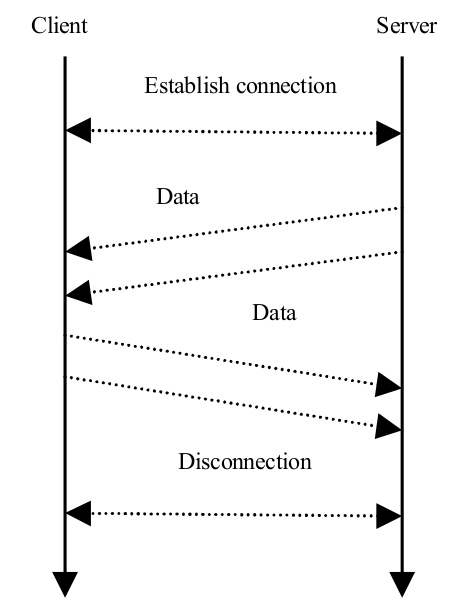
\includegraphics[height=10cm]{Images/C-2/websocket.png}
           		\caption{Model Komunikasi \textit{Websocket}}
           		\label{websocketmodel}
           	\end{figure}
           	\cite{boettiger_introduction_2015}.
		\section{SNMP}
			Simple Network Management Protocol (SNMP) adalah aplikasi pada layer protokol yang digunakan untuk mengatur data pada jaringan. hampir semua vendor jaringan mendukung protokol SNMP. beberapa vendor peralatan telekomunikasi juga mulai didukung oleh protokol SNMP untuk mencapai pengaturan (manajemen) yang terintegrasi. Banyak dari aktivitas manajemen jaringan pada jaringan enterprise yang menggunakan SNMP dalam persentasi yang sangat besar.
			
			SNMP yang berdasarkan paradigma server - client termasuk kedalam manajemen stasiun, agen dan Management Information Bases (MIB). tujuan dari manajemen stasiun adalah untuk mengirimkan request kepada agent dan mengendalikan mereka, manajemen stasiun juga menyediakan antarmuka antara manajer jaringan manusia dan sistem manajemen jaringan. setiap perangkat jaringan memungkinkan untuk mempunyai agen yang dapat mengendalikan basis data dan ketika stasiun manajemen mulai melakukan polling, agen-agen tersebut akan mengirimkan laporan kepada stasiun manajemen.
			
			Dalam pendekatan pemantauan dengan menggunakan SNMP, setiap agen akan mengirimkan stasiun manajemen sebuah informasi melalui polling laporan kejadian. Polling adalah aktivitas untuk melakukan interaksi antara agen dan stasiun manajemen menggunakan metode request dan response. Namun, stasiun manajemen hanya mendengarkan kepada informasi masuk pada pendekatan pelaporan kejadian. Agen akan mengirim informasi kepada stasiun manajemen setiap informasi tersebut dibutuhkan berdasarkan sebuah keputusan.
			
			Pendekatan pemantauan seacar realtime akan didefinisikan sebagai persetujuan antara agen dan stasiun manajemen dimana pada persetujuan semacam in agen harus mengirimkan informasi kepada manajemennya secara berkala tanpa permintaan dari stasiun.
			
			Dalam sebuah kelompak, status dan sifat dari sistem akan dipertimbangkan sebagai pekerjaan memantau dari informasi MIB. tipe data yang akan digunakan untuk memantau lebih penting dibandingkan dengan perancangan jaringan. berikut ini adalah ingormasi yang harus digunakan dalah pemantauan:
			\begin{itemize}
				\item Static: Struktur dan elemen didalam konfigurasi dikategorikan seperti id dari port pada sebuah router atau host. Informasi ini akan jarang berubah.
				\item Dynamic: Informasi kejadian pada jaringan seperti paket dan elemen jaringan
				\item Statistical: Informasi harus berasal dari informasi dinamis seperti rata-rata dari paket yang dikirimkan pada tiap unit.
			\end{itemize}
		\subsection{OID}
			Object Identifier adalah sesuatu untuk mengidentifikasi sebuah objek. Objek ini dapat berupa daerah atau disk drive tunggal. Yang paling umum, didalam IEEE-RAC, adalah OUI (Organizationally Unique Identifier), dan diturunkan secara terorganisasir, dan terdaftar diluar OUI. pengidentifikasi yang paling umum selanjutnya, termasuk pengidentifikasi alamat ethernet adalah pengidentifikasi Extended Unique Identifiers (EUI) atau the World Wide Name (WWN). uniknya, untuk sistem yang sesuai, merupakan properti berharga dalam dua kasus ini. keunikan ini diasumsikan oleh struktur dari nomor unik yang dimulai dengan OUI. IEEE-RAC menetapkan OUI sebagai Object Identifier untuk sebuah organisasi. Object Identifier ini merupakan lapisan didalam konteks yang lebih luas dari pengidentifikasi yang diturunkan secara unik dari titik awal dari sebuah OID, International
			Telecommunication Union Telecommunication Standardization Sector (ITU-T) dan dideskripsikan didalam standar ASN.1. jalur tersebut dilacak menuju ITU-T disebut sebagai "arc" dari sebuah OID. arc ini berkembang menjadi OUI dan RAC lain menetapkan perancang dan melalui penempatan yang dibuat oleh organisasi hingga titik akhir dari sebuah Object Identifier.
			\begin{figure}[H]
				\centering
				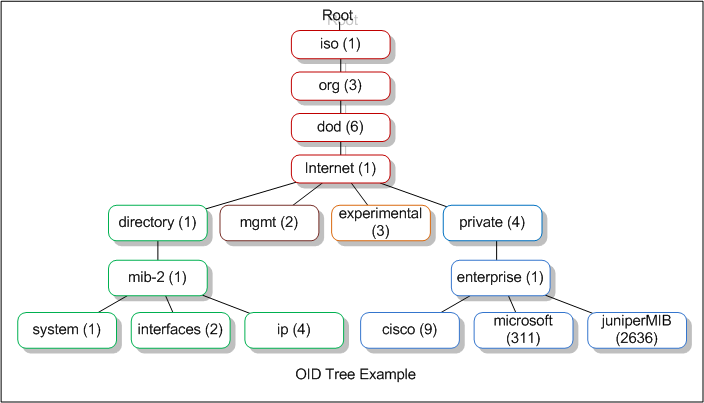
\includegraphics[width=10cm]{Images/C-2/OID.png}
				\caption{Contoh \textit{Object Identifier} (OID)}
				\label{oidexample}
			\end{figure}
		\section{Nagios}
			Nagios adalah perangkat lunak opensource yang aktif dikembangkan, memiliki banyak user juga komunitas yang luas, memiliki banyak plugin tambahan yang dikembangkan oleh user maupun yang terdapat langsung pada awal pengaturan, dan banyak buku tentang Nagios yang diterbitkan. Nagios juga merupakan sistem pemantauan yang paling yang paling populer yang cocok dengan hampir semua distribusi linux. Dukungan komersial tersedia dari perusahaan yang didirikan oleh penciptanya dan pengembang utama sebagai penyedia solusi resmi. Peralatan pemantauan yang berbasis nagios juga tersedia, seperti sensor yang dirancang untuk beroprasi bersama nagios. Karena fleksibilitas dari rancangan perangkat lunak yang menggunakan arsitektur plug-in, layanan pengecekan untuk aplikasi yang pustakanya sudah ditentukan dapat di gunakan. didalam nagios terdapat beberapa plugin lain, seperti script tambahan yang dapat dikostumisasi dan dapat digunakan pada nagios. Nagios adalah program yang ringan dan menyediakan alat pemantauan yang sempurna yang dapat membantu untuk memantau seluruh protokol yang aktif dan perakngkat jaringan yang terhubung dengan topologi. Nagios juga mampu untuk menyediakan grafik yang komperhensif dan bersifat realtime dan analisis tren.
			
		\section{REST API}
			